\newpage \clearpage
\section{Problem \#3}
\label{sec:prob3}

\subsection{Task}
For the 30 stocks that constitute the Dow Jones Industrial Average (Yahoo: DJIA) at the present day: using daily data, estimate the cross correlation over the following periods: 2006 --- 2007, 2008 --- 2009, 2010 --- 2011 and 2012 --- 2013. In all four periods select two stocks that have minimal correlation, construct the equally-weighted portfolio of them and calculate the Sharpe ratio the portfolio.

\subsection{Problem description}

\paragraph*{The Dow Jones Industrial Average}
also called the Industrial Average, the Dow Jones, the Dow Jones Industrial, the Dow 30, or simply the Dow, is a stock market index, and one of several indices created by Wall Street Journal editor and Dow Jones \& Company co-founder Charles Dow. The industrial average was first calculated on May 26, 1896. Currently owned by S\&P Dow Jones Indices, which is majority owned by McGraw-Hill Financial, it is the most notable of the Dow Averages, of which the first (non-industrial) was first published on February 16, 1885. The averages are named after Dow and one of his business associates, statistician Edward Jones. It is an index that shows how 30 large publicly owned companies based in the United States have traded during a standard trading session in the stock market. It is the second oldest U.S. market index after the Dow Jones Transportation Average, which was also created by Dow.

The Industrial portion of the name is largely historical, as many of the modern 30 components have little or nothing to do with traditional heavy industry. The average is price-weighted, and to compensate for the effects of stock splits and other adjustments, it is currently a scaled average. The value of the Dow is not the actual average of the prices of its component stocks, but rather the sum of the component prices divided by a divisor, which changes whenever one of the component stocks has a stock split or stock dividend, so as to generate a consistent value for the index. Since the divisor is currently less than one, the value of the index is larger than the sum of the component prices. Although the Dow is compiled to gauge the performance of the industrial sector within the American economy, the index's performance continues to be influenced by not only corporate and economic reports, but also by domestic and foreign political events such as war and terrorism, as well as by natural disasters that could potentially lead to economic harm.

Along with the NASDAQ Composite, the S\&P 500 Index, and the Russell 2000 Index, the Dow is among the most closely watched U.S. benchmark indices tracking targeted stock market activity. Components of the Dow trade on both the New York Stock Exchange and the NASDAQ. Derivatives of the Dow trade on the Chicago Board Options Exchange and through the CME Group, the world's largest futures exchange company. CME Group owns 24.4\% of S\&P Dow Jones Indices, which maintains the Industrial Average.

To calculate the DJIA, the sum of the prices of all 30 stocks is divided by a divisor, the Dow Divisor. The divisor is adjusted in case of stock splits, spinoffs or similar structural changes, to ensure that such events do not in themselves alter the numerical value of the DJIA. Early on, the initial divisor was composed of the original number of component companies; which made the DJIA at first, a simple arithmetic average. The present divisor, after many adjustments, is less than one (meaning the index is larger than the sum of the prices of the components). That is:
\begin{equation}
DJIA = \frac{\sum p}{d}
\end{equation}
where p are the prices of the component stocks and d is the Dow Divisor.

Events like stock splits or changes in the list of the companies composing the index alter the sum of the component prices. In these cases, in order to avoid discontinuity in the index, the Dow Divisor is updated so that the quotations right before and after the event coincide:
\begin{equation}
DJIA = \frac{\sum p_{old}}{d_{old}} = \frac{\sum p_{new}}{d_{new}}.
\end{equation}
The Dow Divisor is currently 0.15571590501117 as of September 27, 2013. Presently, every \$1 change in price in a particular stock within the average, equates to a 6.42 (1/0.15571590501117) point movement.~\cite{Wiki1}

\paragraph*{Cross-correlation.}

In time series analysis, as applied in statistics and signal processing, the cross correlation between two time series describes the normalized cross covariance function.

Let ($X_t,Y_t$) represent a pair of stochastic processes that are jointly wide sense stationary. Then the cross correlation is given by
\begin{equation}
\gamma_{xy}(\tau) = E[(X_t - \mu_x)(Y_{t+\tau} - \mu_y)],
\end{equation}
where $\mu_x$ and $\mu_y$ are the means of $X_t$ and $Y_t$ respectively.

The cross correlation of a pair of jointly wide sense stationary stochastic process can be estimated by averaging the product of samples measured from one process and samples measured from the other (and its time shifts). The samples included in the average can be an arbitrary subset of all the samples in the signal (e.g., samples within a finite time window or a sub-sampling of one of the signals). For a large number of samples, the average converges to the true cross-correlation. ~\cite{Wiki2}

In this research will be used 3 correlation coefficients: Pearson's correlation coefficient, Spearman's correlation coefficient, Kendall's correlation coefficient.

\textbf{Pearson's} correlation coefficient between two variables is defined as the covariance of the two variables divided by the product of their standard deviations. The form of the definition involves a "product moment", that is, the mean (the first moment about the origin) of the product of the mean-adjusted random variables; hence the modifier product-moment in the name.

Pearson's correlation coefficient when applied to a sample is commonly represented by the letter r and may be referred to as the sample correlation coefficient or the sample Pearson correlation coefficient. We can obtain a formula for r by substituting estimates of the covariances and variances based on a sample into the formula above ~\cite{WikiP}. That formula for r is:
\begin{equation}
r = \frac{\sum ^n _{i=1}(X_i - \bar{X})(Y_i - \bar{Y})}{\sqrt{\sum ^n _{i=1}(X_i - \bar{X})^2} \sqrt{\sum ^n _{i=1}(Y_i - \bar{Y})^2}}
\end{equation}

In statistics, \textbf{Spearman's} rank correlation coefficient or Spearman's rho, named after Charles Spearman and often denoted by the Greek letter $\rho$ (rho) or as $r_s$, is a nonparametric measure of statistical dependence between two variables. It assesses how well the relationship between two variables can be described using a monotonic function. If there are no repeated data values, a perfect Spearman correlation of $+1$ or $-1$ occurs when each of the variables is a perfect monotone function of the other.

The Spearman correlation coefficient is defined as the Pearson correlation coefficient between the ranked variables. For a sample of size $n$, the $n$ raw scores $X_i, Y_i$ are converted to ranks $x_i, y_i$, and $\rho$ is computed from these:
\begin{equation}
 \rho = \frac{\sum_i(x_i-\bar{x})(y_i-\bar{y})}{\sqrt{\sum_i (x_i-\bar{x})^2 \sum_i(y_i-\bar{y})^2}}
\end{equation}
Identical values (rank ties or value duplicates) are assigned a rank equal to the average of their positions in the ascending order of the values ~\cite{WikiS}.

In statistics, the \textbf{Kendall} rank correlation coefficient, commonly referred to as Kendall's tau ($\tau$) coefficient, is a statistic used to measure the association between two measured quantities. A tau test is a non-parametric hypothesis test for statistical dependence based on the tau coefficient.

Specifically, it is a measure of rank correlation, i.e., the similarity of the orderings of the data when ranked by each of the quantities. It is named after Maurice Kendall, who developed it in 1938, though Gustav Fechner had proposed a similar measure in the context of time series in 1897.

Let ($x_1, y_1$), ($x_2, y_2$), �, ($x_n, y_n$) be a set of observations of the joint random variables $X$ and $Y$ respectively, such that all the values of ($x_i$) and ($y_i$) are unique. Any pair of observations ($x_i$, $y_i$) and ($x_j$, $y_j$) are said to be concordant if the ranks for both elements agree: that is, if both $x_i > x_j$ and $y_i > y_j$ or if both $x_i < x_j$ and $y_i < y_j$. They are said to be discordant, if $x_i > x_j$ and $y_i < y_j$ or if $x_i < x_j$ and $y_i > y_j$. If $x_i = x_j$ or $y_i = y_j$, the pair is neither concordant nor discordant.

The Kendall $\tau$ coefficient is defined as:
\begin{equation}
\tau = \frac{(\text{number of concordant pairs}) - (\text{number of discordant pairs})}{\frac{1}{2} n (n-1) }.
\end{equation}

The denominator is the total number pair combinations, so the coefficient must be in the range $-1 <= \tau <= 1$.
\begin{itemize}
\item{If the agreement between the two rankings is perfect (i.e., the two rankings are the same) the coefficient has value 1.}
\item{If the disagreement between the two rankings is perfect (i.e., one ranking is the reverse of the other) the coefficient has value $-1$.}
\item{If X and Y are independent, then we would expect the coefficient to be approximately zero ~\cite{WikiK}.}
\end{itemize}

\paragraph*{Equally-weighted portfolio}
in our case consist only of 2 assets, which has minimal correlation. That's why weights will be equal 50\% for first asset, and 50\% for second.

\paragraph*{Sharpe ratio}
 is a way to examine the performance of an investment by adjusting for its risk. The ratio measures the excess return (or risk premium) per unit of deviation in an investment asset or a trading strategy, typically referred to as risk (and is a deviation risk measure), named after William Forsyth Sharpe.

Since its revision by the original author, William Sharpe, in 1994, the ex-ante Sharpe ratio is defined as:
\begin{equation}
S_p = \frac{E[R_a-R_b]}{\sigma_p} = \frac{E[R_a-R_b]}{\sqrt{\mathrm{var}[R_a-R_b]}},
\end{equation}
where $R_a$ is the asset return, $R_b$ is the return on a benchmark asset, such as the risk free rate of return or an index such as the S\&P 500. $E[R_a-R_b]$ is the expected value of the excess of the asset return over the benchmark return, and $\sigma$ is the standard deviation of this excess return. This is often confused with the information ratio, in part because the newer definition of the Sharpe ratio matches the definition of information ratio within the field of finance. Outside of this field, information ratio is simply mean over the standard deviation of a series of measurements.

The Sharpe ratio characterizes how well the return of an asset compensates the investor for the risk taken. When comparing two assets versus a common benchmark, the one with a higher Sharpe ratio provides better return for the same risk (or, equivalently, the same return for lower risk). However, like any other mathematical model, it relies on the data being correct. Pyramid schemes with a long duration of operation would typically provide a high Sharpe ratio when derived from reported returns, but the inputs are false. When examining the investment performance of assets with smoothing of returns (such as with-profits funds) the Sharpe ratio should be derived from the performance of the underlying assets rather than the fund returns ~\cite{WikiSR}.

\subsection{Solution}
Dow Jones Industrial Average consists of companies with next tickers: AXP, BA, CAT, CSCO, CVX, DD, DIS, GE, GS, HD, IBM, INTC JNJ, JPM, KO, MCD, MMM, MRK, MSFT, NKE, PFE, PG, T, TRV, UNH, UTX, V, VZ, WMT, XOM. Transcription of these tickers (components of DJIA) you can find  \href{http://finance.yahoo.com/q/cp?s=\%5EDJI+Components}{here}. There are no data for Visa until 19th of March 2008. Visa was removed from this list for simplicity. 

2 Yeears Treasury Bonds were choosen as risk free asset. Yields were upload frome \href{http://www.treasury.gov/resource-center/data-chart-center/interest-rates/Pages/TextView.aspx?data=yield}{www.treasury.gov}.Yield, were choosen for last date of each period.

Special function was written on R language, to solve this problem. Input data consists of:
\begin{itemize}
\item{assets returns}
\item{risk free asset returns}
\item{vector of periods}
\item{method to calculate cross-correlations (pearson, spearman, kendall)}
\end{itemize}

On the outpup:
\begin{itemize}
\item{heat maps (cross-correalation matrixes) for 4 periods, saved as pdf files}
\item{cross-correalation matrixes for 4 periods, saved as xlsx-tables}
\item{4 summary text files (for each period), which include tickers for 2 assets with minimal correlation, expected returns of each assets, portfolio expected return, portfolio variance, portfolio Sharpe ratio}

File with code and all data you can find in folder "Problem3".
\end{itemize}

\newpage \clearpage
\subsection{Results}

From the \pref{tab:tab-1}, \pref{tab:tab-2}, \pref{tab:tab-3} you can see portfolios which were constructed for each period and different methods cross--correlation estimation. These assets has minimal covariance for each period. Companies from these portfolios introduce five sectors of economy: finance (GS, JPM), technology (CSCO, VZ), healthcare (UNH), services (WMT), Basic Materials (XOM); and seven industries: Investment Brokerage - National (GS); Networking \& Communication Devices (CSCO); Discount, Variety Stores (WMT); Health Care Plans (UNH); Money Center Banks(JPM); Major Integrated Oil \& Gas (XOM); Telecom Services - Domestic (VZ). The smallest number of full time emloyees has The Goldman Sachs Group, Inc. (32 600 persons). The lagest company for this indicator is Wal-Mart Stores Inc. (2 000 000 persons).

%%%%%%%%%%%%%Pearson's cross-correlation%%%%%%%%%%%%%%%%%%%%%%%%%%%
As you can see, all companies in each portfolio introduce different sectors (it is quite logical, cause the reason we choose these portfolio was minimal covariance between assets). Cross--correalation matrices as a heat maps introduce in \pref{fig:f1} --- \pref{fig:f12}

\begin{table}[ht]
\caption{Portfolio based on Pearson's cross-correlation}
\begin{tabular}{|p{3cm}|p{5.5cm}| p{5.5cm}|}
	\hline
	\textbf{\ Period} & {\ Asset 1} & {\ Asset 2}\\
	\hline {\ 2006--2007 } & {\ UnitedHealth Group Incorporated (UNH)} & {\ Cisco Systems, Inc.(CSCO)} \\
	\hline {\ 2008--2009} & {\ UnitedHealth Group Incorporated (UNH)} & {\ JPMorgan Chase \& Co. (JPM)} \\
	\hline {\ 2010--2011} & {\ Wal-Mart Stores Inc. (WMT)} & {\ The Goldman Sachs Group, Inc. (GS)} \\
	\hline {\ 2012--2013} & {\ Wal-Mart Stores Inc. (WMT)} & {\ Cisco Systems, Inc. (CSCO)} \\
	\hline
\end{tabular}
\label{tab:tab-1}
\end{table}

From \pref{fig:f1}, \pref{fig:f2} you can see that UnitedHealth Group Incorporated (UNH) uncorrelated almost all companies in DJIA.

\begin{figure}
	\centering
	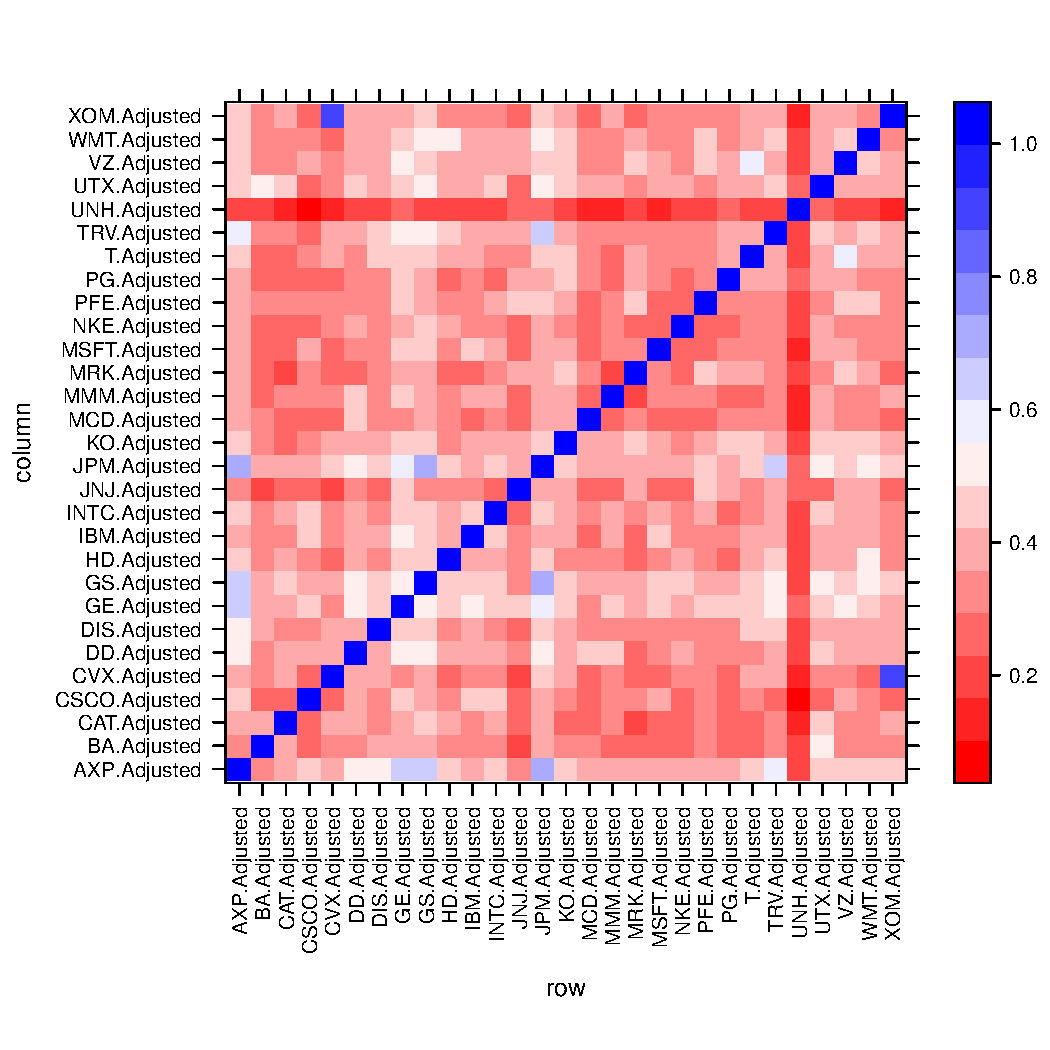
\includegraphics[width=0.6\textwidth,clip,keepaspectratio]{src/Pearson/pearson_2006-01-01_2007-12-31.pdf}
	\caption{Pearson's cross--correlation matrix for period since 2006-01-01 to 2007-12-31}
	\label{fig:f1}
\end{figure}

\begin{figure}
	\centering
	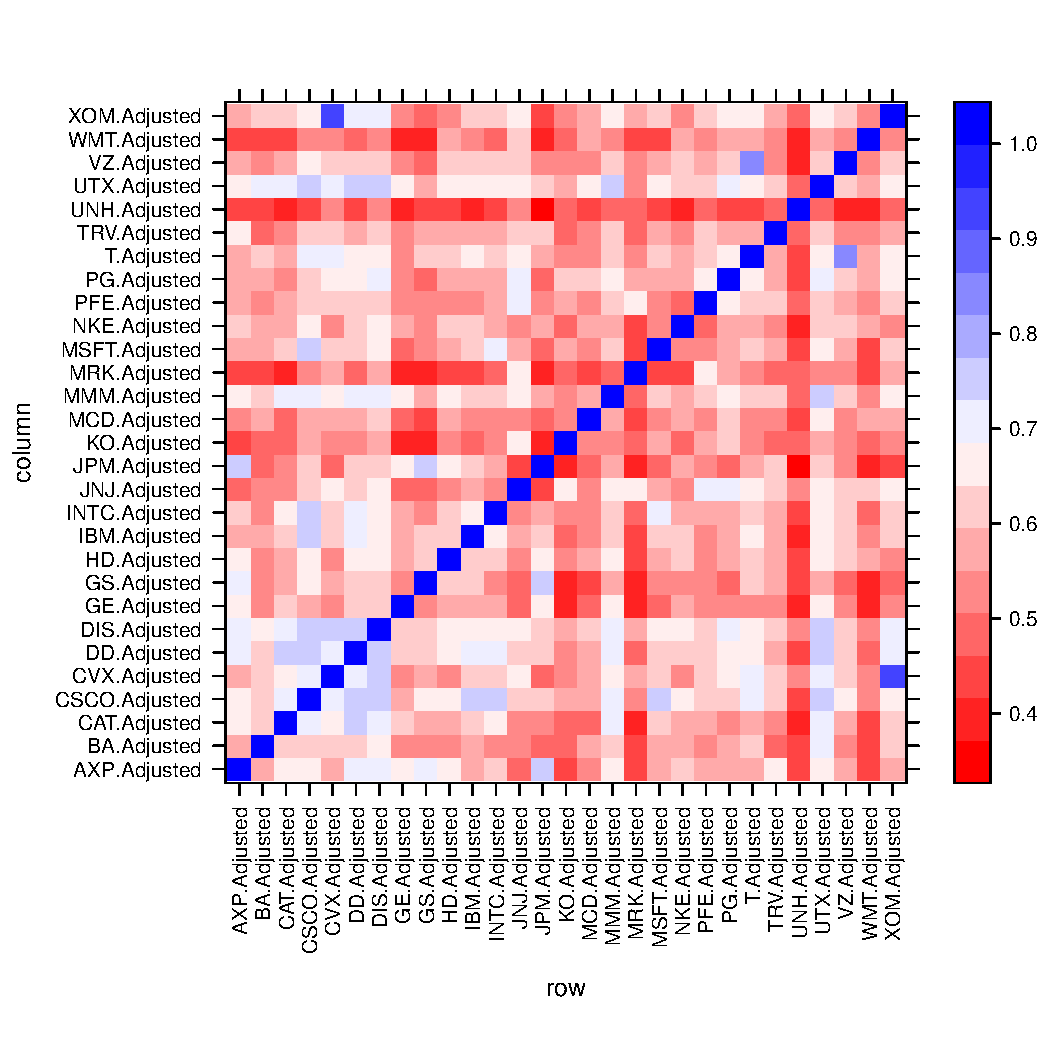
\includegraphics[width=0.6\textwidth,clip,keepaspectratio]{src/Pearson/pearson_2008-01-01_2009-12-31.pdf}
	\caption{Pearson's cross--correlation matrix for period since 2008-01-01 to 2009-12-31}
	\label{fig:f2}
\end{figure}

For periods which described by \pref{fig:f3}, \pref{fig:f4} (2010 -- 2014), you can see changes in cross-correlation matrices. The Goldman Sachs Group, Inc. (GS), Cisco Systems, Inc. (CSCO) and Wal-Mart Stores Inc. (WMT), uncorrelatad with companies in DJIA.

\begin{figure}
	\centering
	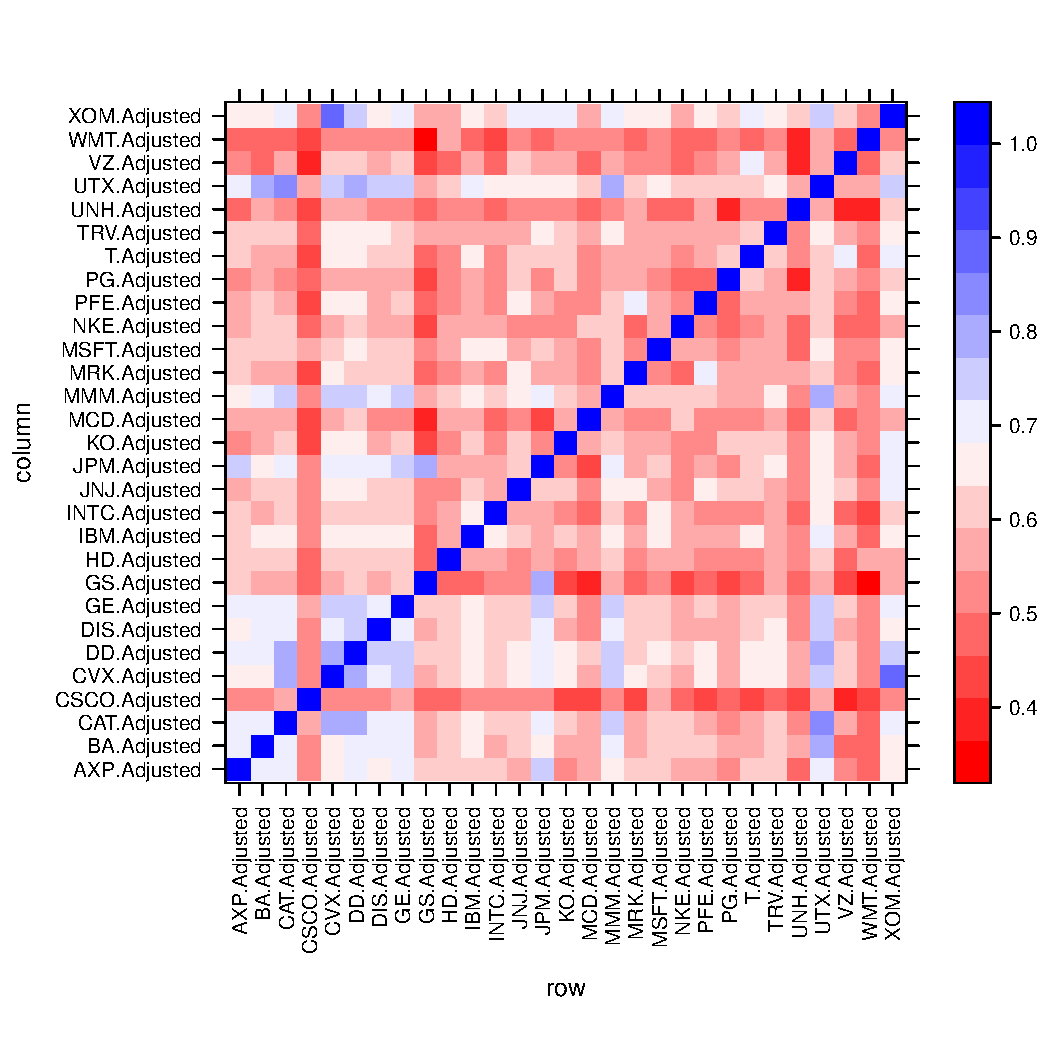
\includegraphics[width=0.6\textwidth,clip,keepaspectratio]{src/Pearson/pearson_2010-01-01_2011-12-31.pdf}
	\caption{Pearson's cross--correlation matrix for period since 2010-01-01 to 2011-12-31}
	\label{fig:f3}
\end{figure}

\begin{figure}
	\centering
	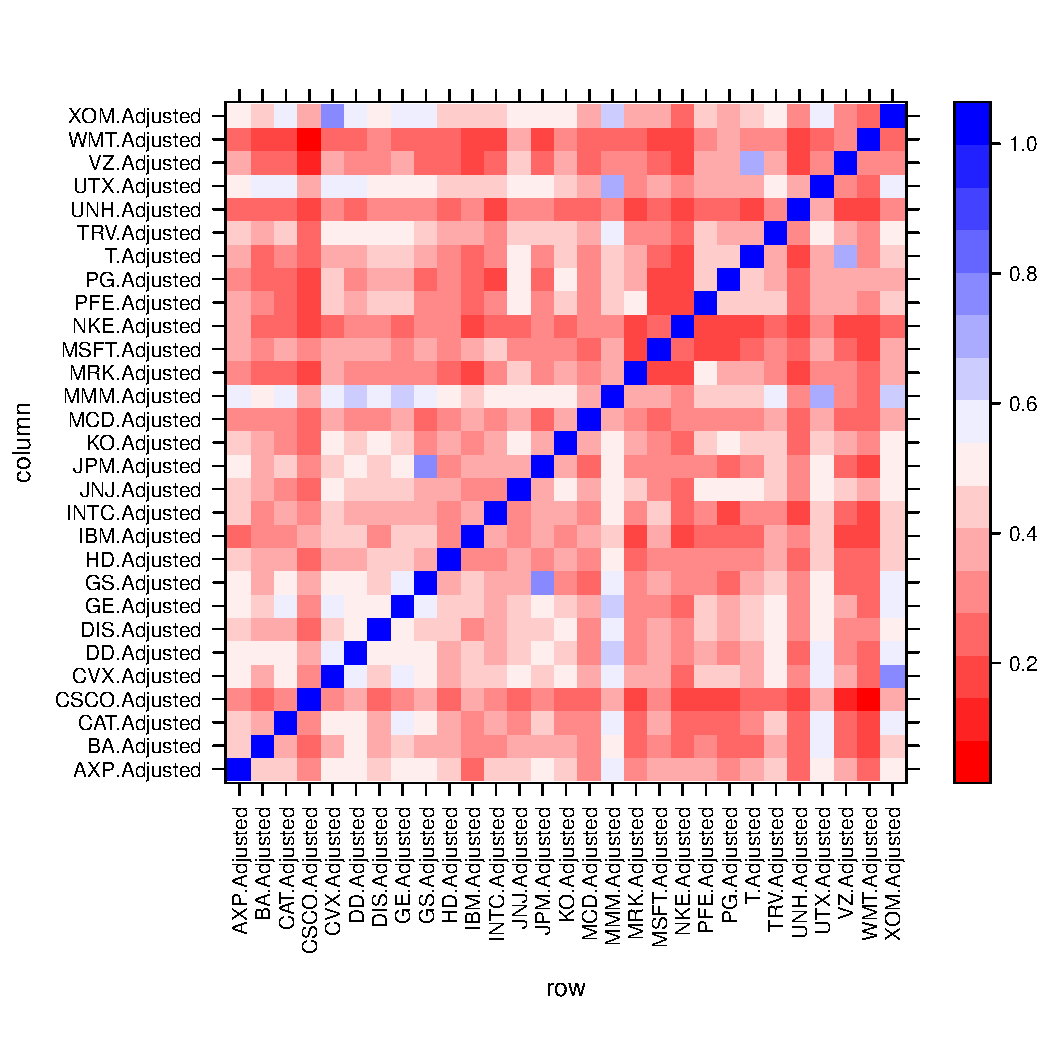
\includegraphics[width=0.6\textwidth,clip,keepaspectratio]{src/Pearson/pearson_2012-01-01_2013-12-31.pdf}
	\caption{Pearson's cross--correlation matrix for period since 2012-01-01 to 2013-12-31}
	\label{fig:f4}
\end{figure}



%%%%%%%%%%%%%Spearman's cross-correlation%%%%%%%%%%%%%%%%%%%%%%%%%%%
\newpage \clearpage
Portfolio, which based on Spearman's cross-correlation save properties of the Pearson's cross--correlatin based portfolio for first two periods (\pref{fig:f5}, \pref{fig:f6}). UnitedHealth Group Incorporated (UNH) uncorrelated almost all companies in DJIA.

\begin{table}
\caption{Portfolio based on Spearman's cross-correlation}
\begin{tabular}{|p{3cm}|p{5.5cm}| p{5.5cm}|}
	\hline
	\textbf{\ Period} & {\ Asset 1} & {\ Asset 2}\\
	\hline {\ 2006--2007 } & {\ UnitedHealth Group Incorporated (UNH)} & {\ Exxon Mobil Corporation (XOM)} \\
	\hline {\ 2008--2009} & {\ UnitedHealth Group Incorporated (UNH)} & {\ Verizon Communications Inc. (VZ)} \\
	\hline {\ 2010--2011} & {\ Wal-Mart Stores Inc. (WMT)} & {\ The Goldman Sachs Group, Inc. (GS)} \\
	\hline {\ 2012--2013} & {\ Verizon Communications Inc. (VZ)} & {\ Cisco Systems, Inc. (CSCO)} \\
	\hline
\end{tabular}
\label{tab:tab-2}
\end{table}

\begin{figure}
	\centering
	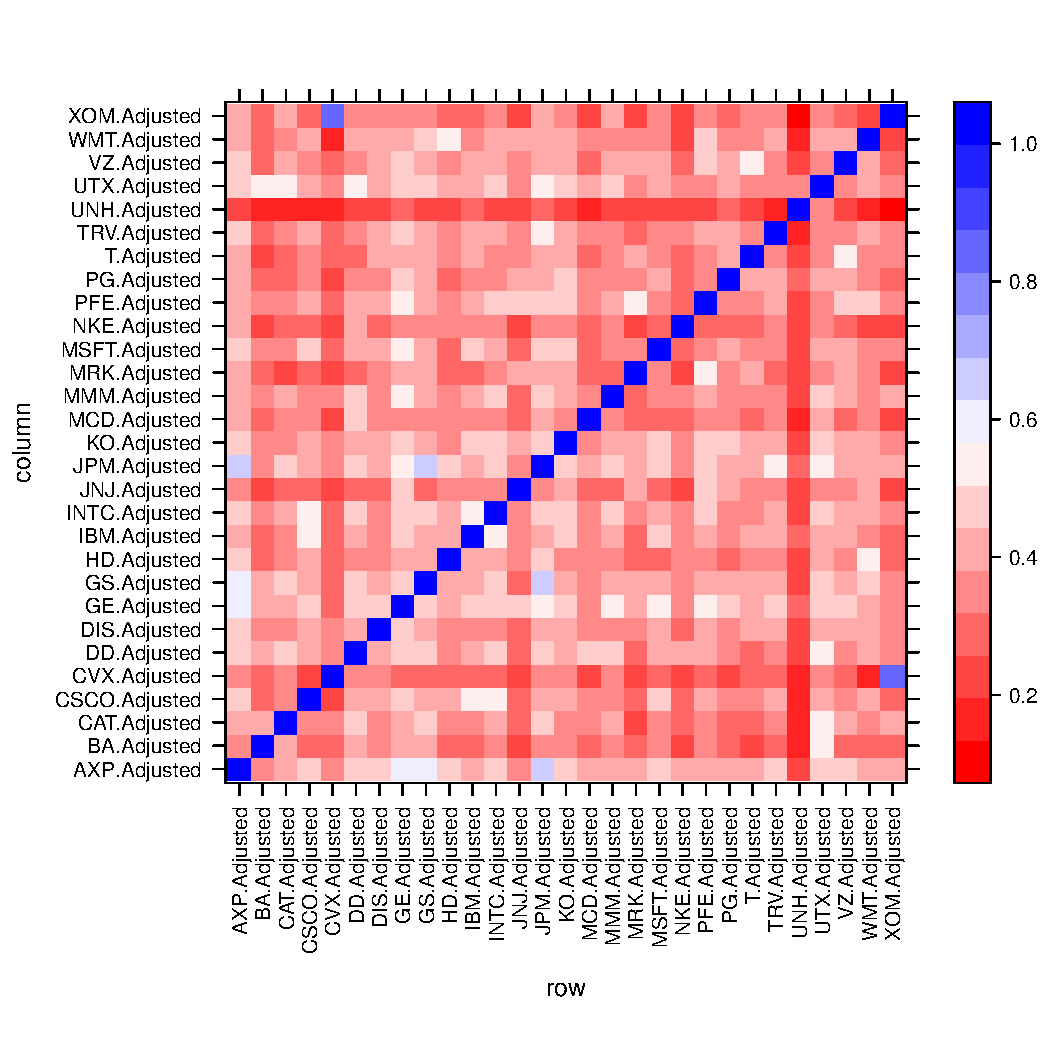
\includegraphics[width=0.6\textwidth,clip,keepaspectratio]{src/Spearman/spearman_2006-01-01_2007-12-31.pdf}
	\caption{Spearman's cross--correlation matrix for period since 2006-01-01 to 2007-12-31}
	\label{fig:f5}
\end{figure}

\begin{figure}
	\centering
	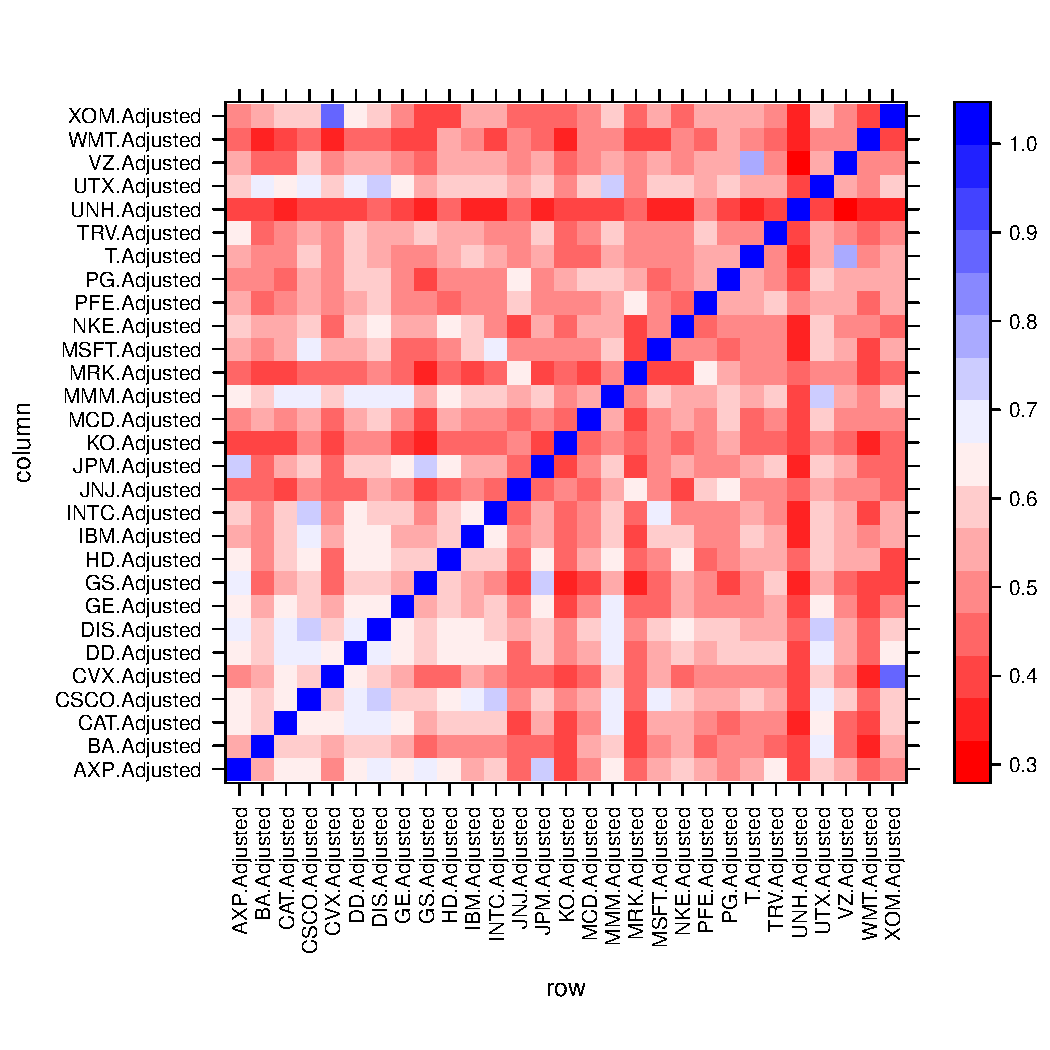
\includegraphics[width=0.6\textwidth,clip,keepaspectratio]{src/Spearman/spearman_2008-01-01_2009-12-31.pdf}
	\caption{Spearman's cross--correlation matrix for period since 2008-01-01 to 2009-12-31}
	\label{fig:f6}
\end{figure}

Third period (2010--2011) only Wal-Mart Stores Inc. (WMT), was differ much from all list of DJIA index. Correlation was higher beetween all companies this period. The reason of it, we think, is consequences of the World Financia Crisis which begans at 2008. Economies of big amount of countries were in recession.

The global recession resulted in a sharp drop in international trade, rising unemployment and slumping commodity prices. Several economists predicted that recovery might not appear until 2011 and that the recession would be the worst since the Great Depression of the 1930s. Paul Krugman, who won the Nobel Memorial Prize in Economics, once commented on this as seemingly the beginning of "a second Great Depression. "The conditions leading up to the crisis, characterised by an exorbitant rise in asset prices and associated boom in economic demand, are considered a result of the extended period of easily available credit and inadequate regulation and oversight.~\cite{WikiWC}

\begin{figure}
	\centering
	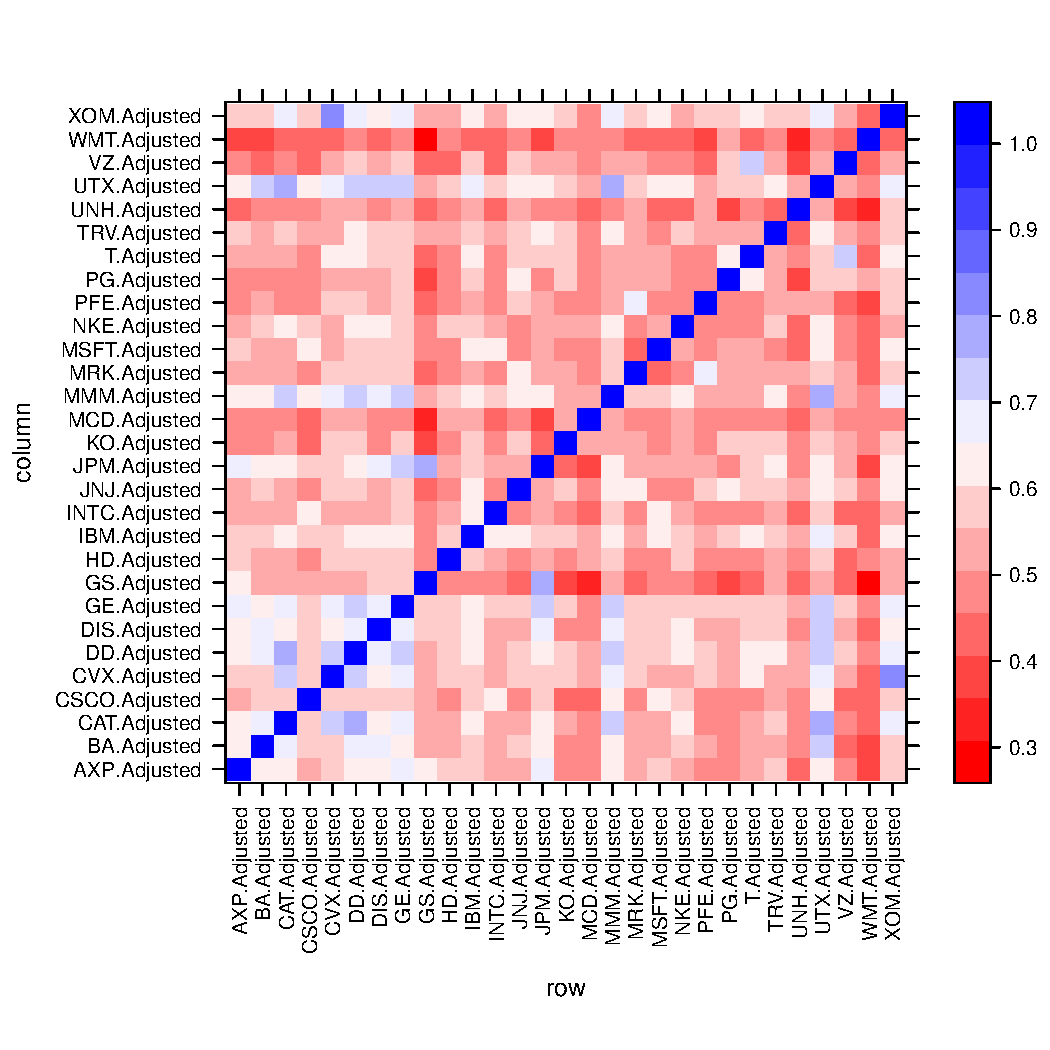
\includegraphics[width=0.6\textwidth,clip,keepaspectratio]{src/Spearman/spearman_2010-01-01_2011-12-31.pdf}
	\caption{Spearman's cross--correlation matrix for period since 2010-01-01 to 2011-12-31}
	\label{fig:f7}
\end{figure}

\begin{figure}
	\centering
	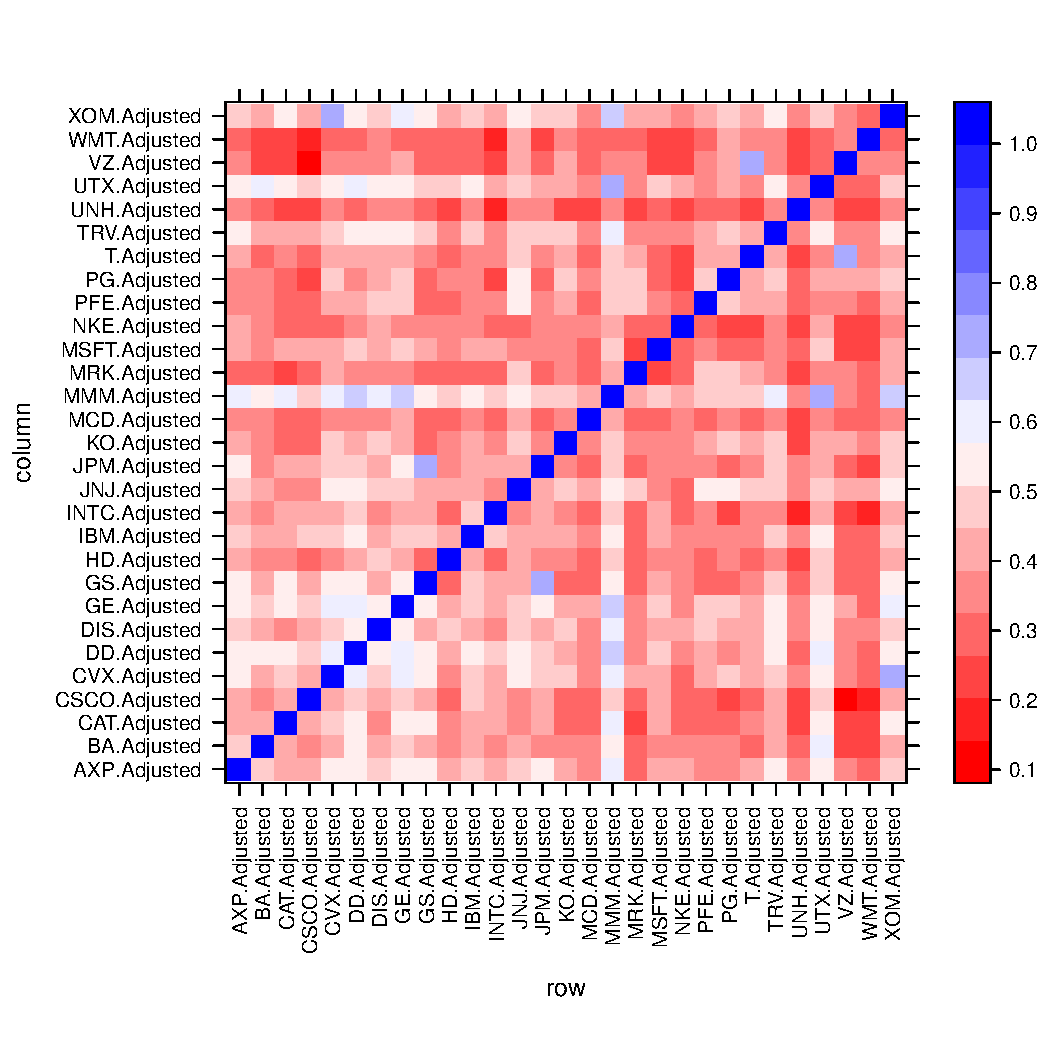
\includegraphics[width=0.6\textwidth,clip,keepaspectratio]{src/Spearman/spearman_2012-01-01_2013-12-31.pdf}
	\caption{Spearman's cross--correlation matrix for period since 2012-01-01 to 2013-12-31}
	\label{fig:f8}
\end{figure}



%%%%%%%%%%%%%Kendall's cross-correlation%%%%%%%%%%%%%%%%%%%%%%%%%%%
\newpage \clearpage

Protfolio, which build with Kendall's cross-correlation very close to portfolio which build with Sperman's cross-correlation. Differ is on  period from 2008--2009. If you see to heet maps \pref{fig:f9} -- \pref{fig:f12}, the asset more uncorrelated versus Pearson and Spearman correlation.

\begin{table}
\caption{Portfolio based on Kendall's cross-correlation}
\begin{tabular}{|p{3cm}|p{5.5cm}| p{5.5cm}|}
	\hline
	\textbf{\ Period} & {\ Asset 1} & {\ Asset 2}\\
	\hline {\ 2006--2007 } & {\ UnitedHealth Group Incorporated (UNH)} & {\ Exxon Mobil Corporation (XOM)} \\
	\hline {\ 2008--2009} & {\ UnitedHealth Group Incorporated (UNH)} & {\ Wal-Mart Stores Inc. (WMT)} \\
	\hline {\ 2010--2011} & {\ Wal-Mart Stores Inc. (WMT)} & {\ The Goldman Sachs Group, Inc. (GS)} \\
	\hline {\ 2012--2013} & {\ Verizon Communications Inc. (VZ)} & {\ Cisco Systems, Inc. (CSCO)} \\
	\hline
\end{tabular}
\label{tab:tab-3}
\end{table}

\begin{figure}
	\centering
	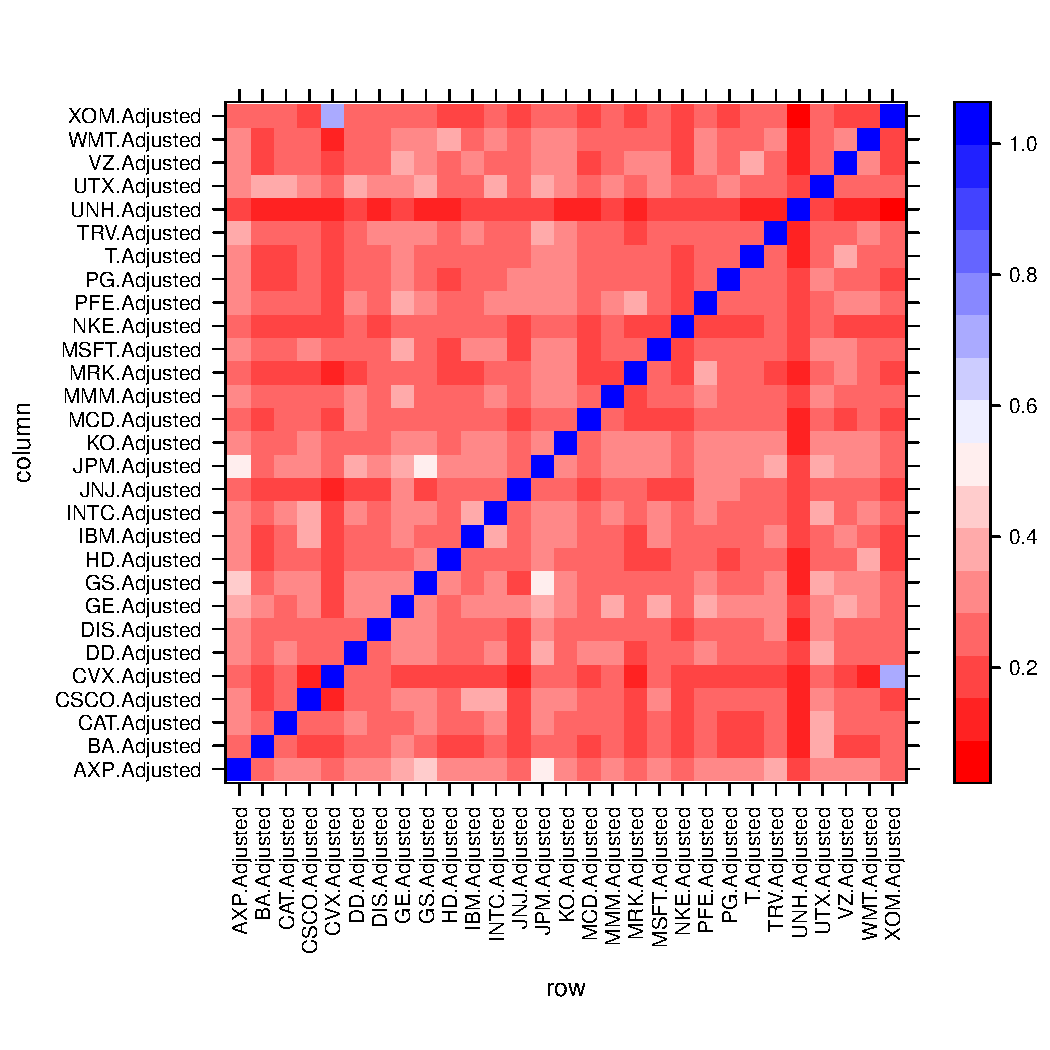
\includegraphics[width=0.5\textwidth,clip,keepaspectratio]{src/Kendall/kendall_2006-01-01_2007-12-31.pdf}
	\caption{Kendall's cross--correlation matrix for period since 2006-01-01 to 2007-12-31}
	\label{fig:f9}
\end{figure}

\begin{figure}
	\centering
	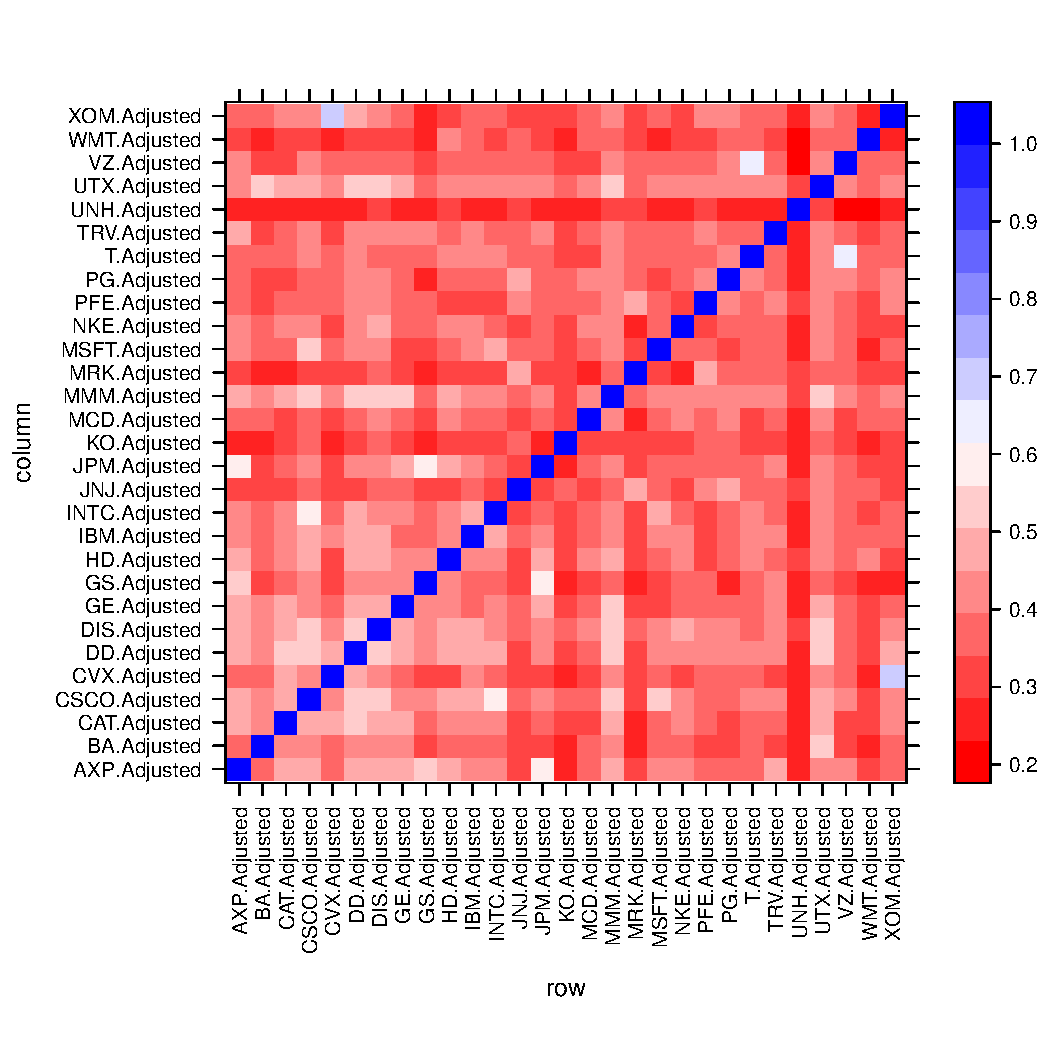
\includegraphics[width=0.6\textwidth,clip,keepaspectratio]{src/Kendall/kendall_2008-01-01_2009-12-31.pdf}
	\caption{Kendall's cross--correlation matrix for period since 2008-01-01 to 2009-12-31}
	\label{fig:f10}
\end{figure}

\begin{figure}
	\centering
	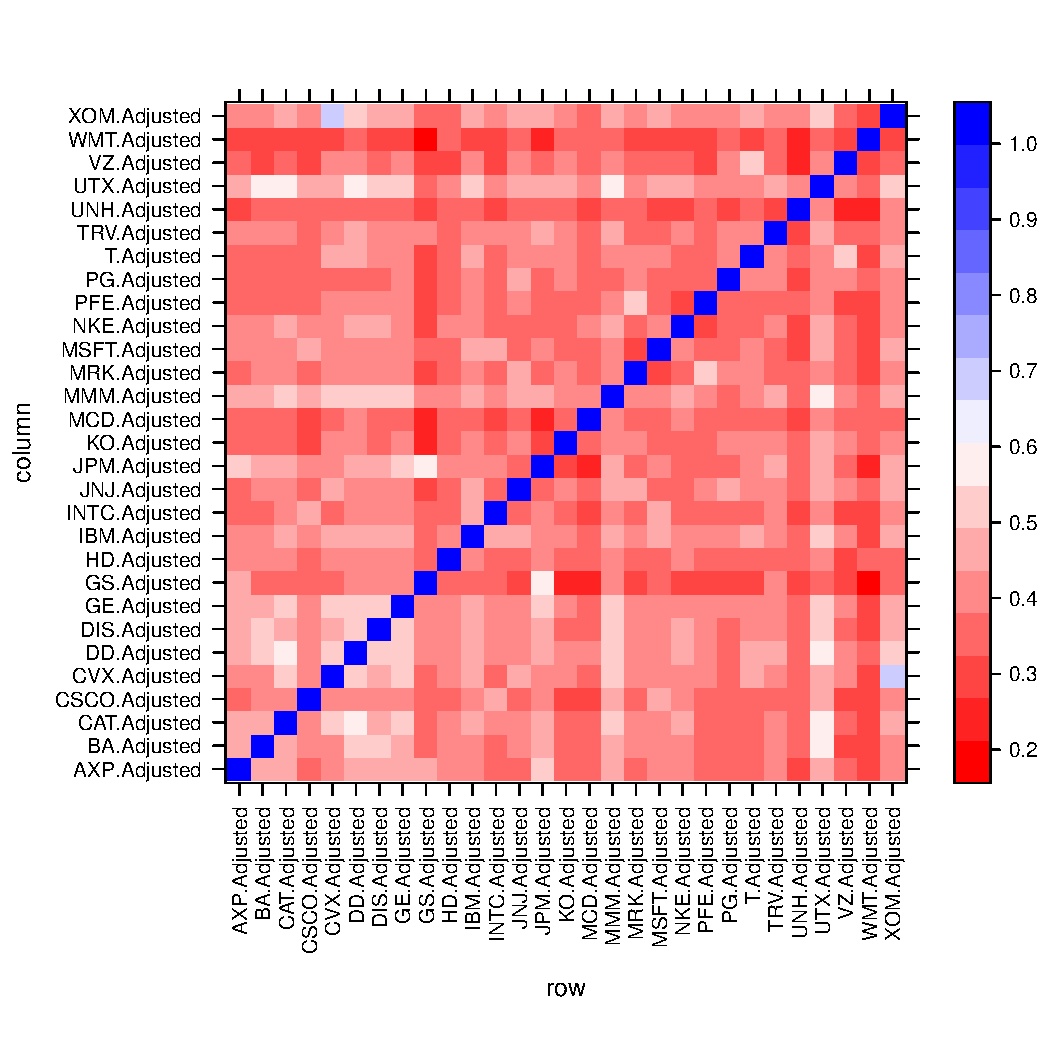
\includegraphics[width=0.6\textwidth,clip,keepaspectratio]{src/Kendall/kendall_2010-01-01_2011-12-31.pdf}
	\caption{Kendall's cross--correlation matrix for period since 2010-01-01 to 2011-12-31}
	\label{fig:f11}
\end{figure}

\begin{figure}
	\centering
	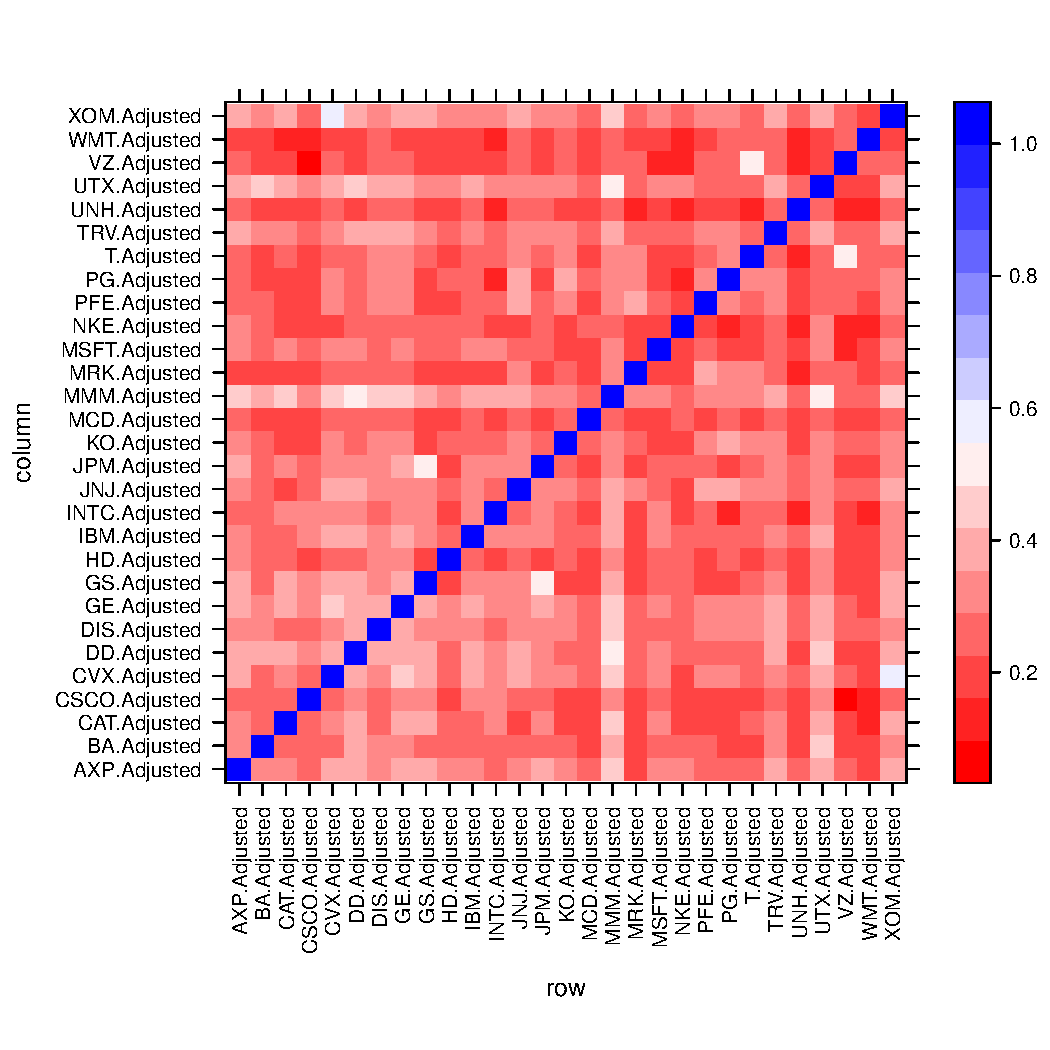
\includegraphics[width=0.6\textwidth,clip,keepaspectratio]{src/Kendall/kendall_2012-01-01_2013-12-31.pdf}
	\caption{Kendall's cross--correlation matrix for period since 2012-01-01 to 2013-12-31}
	\label{fig:f12}
\end{figure}

%%%%%%%%%%%%%%%%%%%%%%%%%%%%%%Sharp ratio%%%%%%%%%%%%
If you see to \pref{tab:tab-4}, portfolios which calculates by Spearman's and Kendall's are equall. But portfolios which calculates by Pearson method. It means that last portfolio has the same yield with less risk. But we should understand, that Person cross--correlation \textbf{not robust} and it isn't efficient if returns has not normal distribution.


\begin{table}
\caption{Portfolio's Sharpe ratio for four periods}
\begin{tabular}{|p{4cm}|p{3cm}| p{3cm}|p{3cm}|}
	\hline
	\textbf{\ Period} & {\ Pearson} & {\ Speaman} & {\ Kendall}\\
	\hline {\ 2006--2007 } & {\ -0.044} & {\ -0.048} & {\ -0.048}\\
	\hline {\ 2008--2009} & {\ -0.006} & {\ -0.009} & {\ -0.009}\\
	\hline {\ 2010--2011} & {\ -0.004} & {\ -0.005} & {\ -0.005}\\
	\hline {\ 2012--2013} & {\ -0.004} & {\ -0.004} & {\ -0.004}\\
	\hline
\end{tabular}
\label{tab:tab-4}
\end{table}




























